\apendice{Documentación técnica de programación}
En este apéndice, incluiremos las bases de programación y desarrollo del proyecto necesarias para un buen funcionamiento del Sistema de Recomendación. 

\section{Recogida de datos}
La recogida de datos se desarrolla utilizando un cuestionario anónimo en web, utilizando la página Typeform, de forma que se deben introducir de forma obligatoria las calificaciones de los tres primeros cursos. En este proyecto, hasta la fecha, 56 alumnos y ex-alumnos han rellenado dicho cuestionario. 
\subsection{Creación del cuestionario}
El cuestionario se ha creado utilizando la página gratuita de Typeform, modificando el aspecto del cuestionario y añadiendo las asignaturas y sus restricciones. 
Se procedió al  guardado de los ficheros en un documento Excel en Google Drive, denominado "DatosTFG\_SistemasRecomendacion". 

\subsection{Obtención de los datos}
Para obtener los datos almacenados en Drive, se ha necesitado activar el API GoogleDrive, para poder acceder a los datos sin necesidad de descargar continuamente el fichero. Para ello: 
\begin{itemize}
 
\item Acceder a \url{https://console.developers.google.com/apis/library}
\item Crear un nuevo proyecto\ref{fig:D.1.1}. Se debe tener en cuenta que hay un número máximo de proyectos creados de forma gratuita.
\begin{figure}[h]
\centering
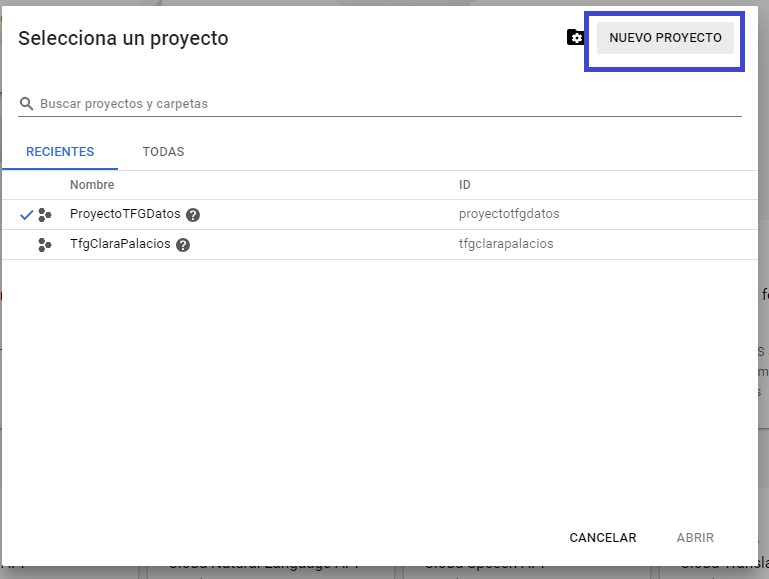
\includegraphics[width=0.90\textwidth]{crear_proyecto_api}
\caption{Crear proyecto nuevo}
\label{fig:D.1.1}
\end{figure}  
\item Introducir el nombre del proyecto creado y pulsar Crear.\ref{fig:D.1.2} 
\begin{figure}[h]
\centering
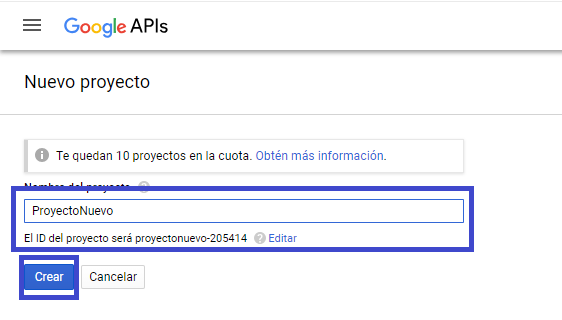
\includegraphics[width=0.90\textwidth]{nombre_proyecto_api}
\caption{Dar nombre al proyecto}
\label{fig:D.1.2}
\end{figure}  
\item Acceder a \url{https://console.developers.google.com/}
\item Buscar GoogleDrive Api, y activar dicha api.\ref{fig:D.1.3} 
\begin{figure}[h]
\centering
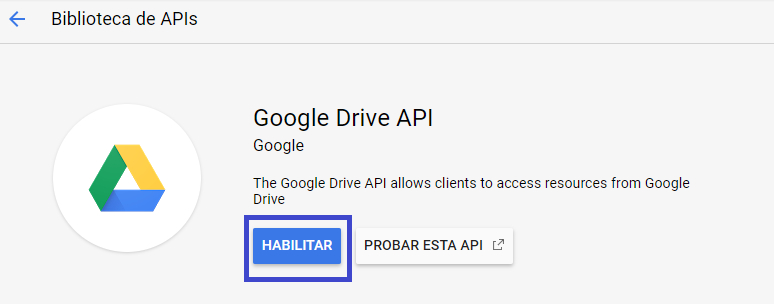
\includegraphics[width=0.90\textwidth]{activar_google_drive}
\caption{Activar Google Drive}
\label{fig:D.1.3}
\end{figure}  
\item Activar credenciales para el proyecto creado\ref{fig:D.1.3} 
\begin{figure}[h]
\centering
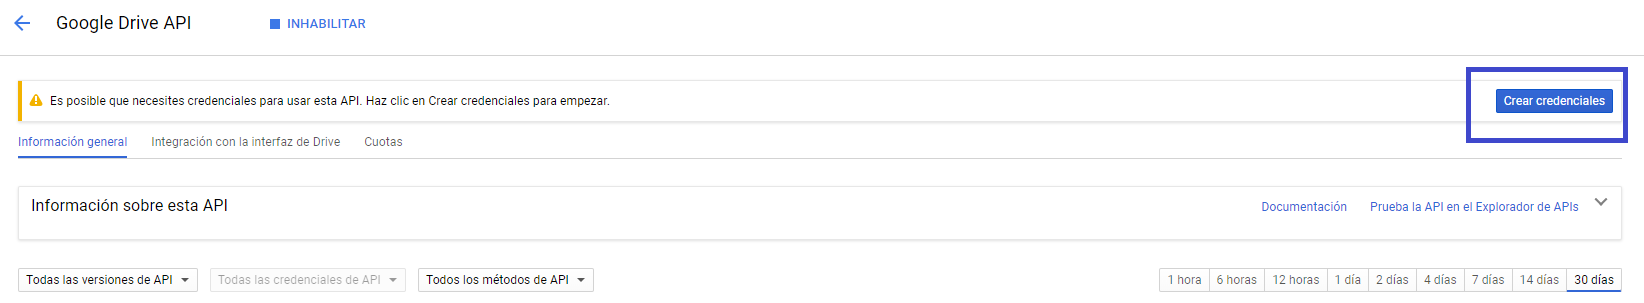
\includegraphics[width=0.90\textwidth]{credenciales_proyecto_api}
\caption{Obtener Credenciales}
\label{fig:D.1.3}
\end{figure}  
\item Activar las credenciales para acceder al documento en Google Drive. \ref{fig:D.1.4} De esta forma, un cliente puede acceder a dichos datos. (El administrador en este caso). Pulsar "Qué credenciales necesito"
\begin{figure}[h]
\centering
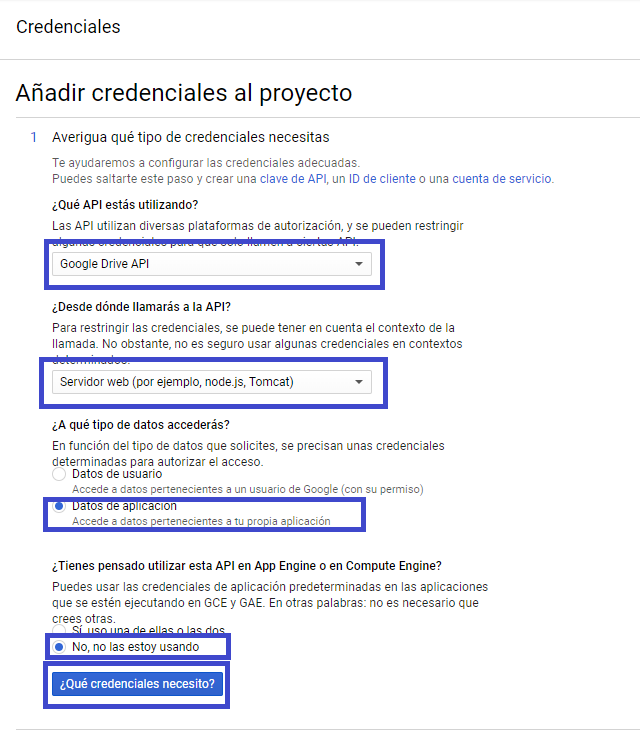
\includegraphics[width=0.90\textwidth]{credenciales_seleccionar_api}
\caption{Activar Credenciales}
\label{fig:D.1.4}
\end{figure}  
\item Introducir el rol que se le dará, así como el nombre del servicio. \ref{fig:D.1.5}
\begin{figure}[h]
\centering
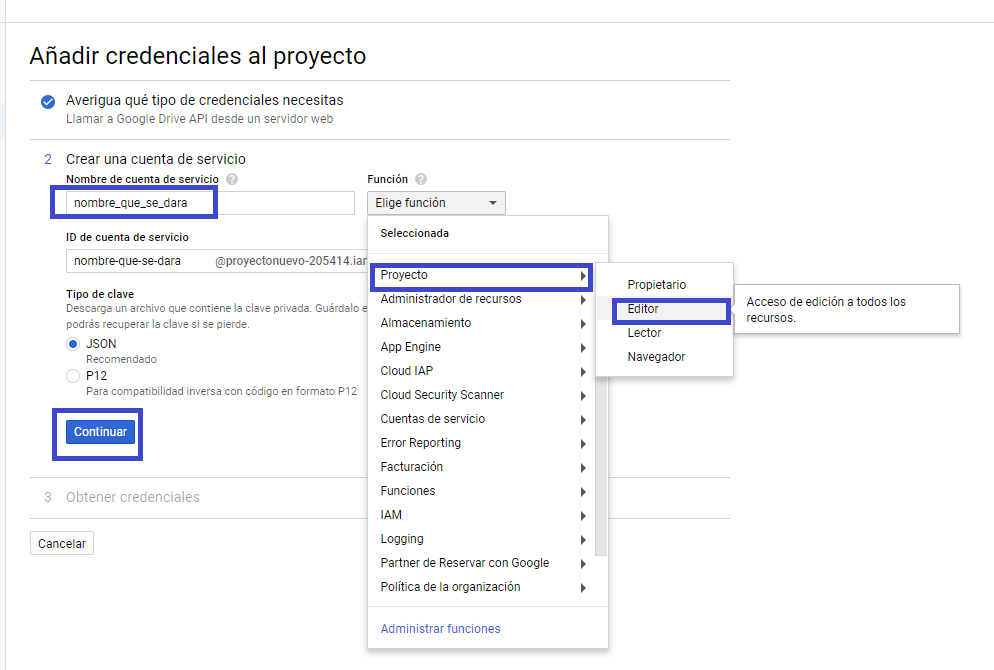
\includegraphics[width=0.90\textwidth]{nombre_rol_api}
\caption{Introducir nombre y rol}
\label{fig:D.1.5}
\end{figure}
\item Tras pulsar continuar, se descargará un fichero json, y mostrará un mensaje por pantalla. 
\item Abrir el fichero json y copiar el correo electrónico obtenido, compartiéndolo en el documento existente en google drive. 
\end{itemize}
Una vez pudiendo acceder a dichos datos, se debe acceder desde el código utilizando la librería ServiceAccountCredentials. Se debe tener en cuenta que el fichero json debe de encontrarse en el mismo directorio que el código que desee acceder al mismo. 


\section{Tratamiento de los datos}
Los datos recibidos desde la API contienen columnas no necesarias para el proyecto, tales como el Token y la fecha de rellenado. Por otra parte, al recibir los datos, en caso de no haberse cursado, el valor será un string vacío, por lo que habrá que modificar ese string por un NaN (de la librería numpy), para diferenciar de las calificaciones marcadas con cero por los usuarios.   Los datos devueltos por esta función de tratamiento se almacenan en un dataframe

\section{Sistemas de recomendación}
El desarrollo de los sistemas de recomendación se simplifica reutilizando las funciones de cálculo de matriz de similitud y de matriz de distancias, realizándolas de forma genérica para evitar la duplicidad del código. 
\subsection{Basado en usuarios y productos}
Se recibe la matriz de similitud y el diccionario de las asignaturas de 4 para calcular la predicción de las asignaturas y devolvérselas. 

\subsection{Util}
El paquete util implementa tanto el coeficiente de Pearson como la matriz de similitud. 
\subsubsection{Distancias}
Par el cálculo del coeficiente de pearson se recibe el dataframe junto con las variables a y b, que en uno de los filtros colaborativos son usuarios mientras que en el otro son items. De esta forma, el código puede ser reutilizado para ambos sistemas de recomendación. 
\subsubsection{Matriz\_Similitud}
En la misma línea, el cálculo de la matriz de similitud se realiza de forma genérica para poder acceder tanto por el filtro colaborativo basado en usuarios como por el filtro colaborativo basado en productos. Esta clase recibe el dataframe de los datos con los que se trabajará, calcula la matriz de similitud con todos los elementos y devuelve una matriz de similitud elemento-elemento. 

\section{I\_O\_Datos}
El paquete I\_O\_Datos implementa la recuperación de datos tanto de drive, de un fichero binario o de la base de datos. De esta forma:
\subsection{Binario}
Para la lectura de datos en binario, se obtiene todo el dataframe eliminándose las columnas innecesarias,  y devolviéndose un dataframe con el que se pueda trabajar. 

\subsection{GoogleDrive}
El funcionamiento de esta opción se ha realizado en la primera sección de forma que no se entrará en detalles

\subsection{API\_Rest}
En esta clase, se obtienen-a través de un json- y se almacenan los datos de Cloud reemplazando tildes y espacios en blanco de los nombres de las asignaturas. Por otra parte, se deben eliminar las columnas no necesarias. 
Finalmente, la clase devuelve un dataframe para poder trabajar con él. 

\section{Diccionario}
El diccionario utilizado sirve tanto para los elementos de la interfaz gráfica (secciones, botones...) como el almacenamiento y subdivisión de las asignaturas por semestres, así como la caracterización de las asignaturas. 

\section{Interfaz gráfica}
La interfaz gráfica se ha desarrollado utilizando PyQt5. Para su estructura, se ha subdividido el código en paquetes, de forma haya un paquete por cada pestaña y un panel de pestañas y la ventana principal. 
\subsection{Asignaturas}
Este paquete contienen las asignaturas de cada curso para la primera pestaña, junto con los layout y checkbox para modificar sus ponderaciones. Por otra parte, la clase ``Asignatura'' Implementa los métodos de guardado de los datos y carga de los mismos. 

\subsection{Modelos}
Este paquete implementa las clases para la muestra de los resultados de las asignaturas, así como las gráficas relacionadas con dichos resultados. Esto está implementado en la clase TopCuartoFrame, clase encargada de pintar los resultados. \\Para su obtención, desde la clase Modelos del mismo paquete se implementan las funciones para ejecutar los filtros colaborativos y establecer las asignaturas del curso que vayan a aparecer en la pestaña. 

\subsection{Estadísticas}
Corresponde con la tercera pestaña de gráficos auxiliares para el usuario. Este paquete contiene los cuatro cursos para mostrar sus nombres en el área de las leyendas y su media, mediana, máximo y mínimo en las gráficas. Estos cálculos se realizan en el paquete estadística, así como el establecimiento de las barras verticales correspondientes a las asignaturas.


\section{Base de Datos} 